\section{Reconstrucción continua de señales muestreadas}

\subsection{Reconstrucción ideal}

\begin{frame}
\frametitle{Reconstrucción ideal I}

\vspace{-0.2cm}

\footnotesize
\begin{itemize}
\item Señal banda limitada: \alert{$X_c(jw)=0$ para $|w|>w_M$}

\item Señal muestreada idealmente: \alert{$x_p(t)\!=\!x_c(t)\!\cdot \! \sum_{k=-\infty}^{\infty}\! \!\delta(t-kT_s)$}

\item CTFT señal muestreada idealmente: \alert{$X_p(jw)\!\!=\!\!\frac{1}{T_s}\!\! \sum_{k=-\infty}^{\infty}\!X_c(j(w\!-\!kw_s))$}
\end{itemize}



\hspace{1.0cm}\alert{¿Reconstrucción de la señal original a partir de la muestreada?}


\vspace{-0.3cm}

\footnotesize
\begin{columns}[c]
\begin{column}{4.5cm}
\visible<2->{\includegraphics[width=4.5cm]{./Figures/RecIdeal.ps}}
\end{column}
\begin{column}{7cm}
\begin{itemize}

\visible<3->{
\item Respuesta en dominio frecuencia:

$Y(jw)=H(jw)\cdot X_p(jw)$}

\visible<4->{
\item Filtro paso bajo ideal:

$H(jw)=T_s \Pi (\frac{w}{2w_c})$ 

\hspace{0.3cm} con $w_M\!<\!w_c\!<\!w_s\!-\!w_M$

$Y(jw)=H(jw)\cdot X_p(jw)=X_c(jw)$}


\visible<5->{
\item Respuesta en dominio temporal:

$y(t)=(h*x_p)(t)$}

\visible<6->{
\item Función Ponderatriz del Filtro:

$Sa(\frac{t}{2}) \rightarrow 2 \pi \Pi(w)$

$Sa(\frac{2w_ct}{2}) \rightarrow \frac{2 \pi}{2w_c} \Pi(\frac{w}{2w_c}) \rightarrow \frac{\pi}{w_c} \Pi(\frac{w}{2w_c}) $

$h(t)=\frac{T_s w_c}{\pi}Sa(w_ct)$
}


\end{itemize}
\end{column}

\end{columns}


\end{frame}

%%%%%%%%%%%%%%%%%

\begin{frame}
\frametitle{Reconstrucción ideal II}

\footnotesize

\begin{itemize}

\color{gray}

\item Señal original  $x_c(t)$ de banda limitada ($X_c(w)=0$ para $|w|>w_m$)

\item Señal muestreada idealmente: $x_p(t)\!=\!x_c(t)\!\cdot \! \sum_{k=-\infty}^{\infty}\! \!\delta(t-kT_s)$

\item Función ponderatriz del filtro: $h(t)=\frac{T_s w_c}{\pi}Sa(w_ct)$


\item Salida del filtro: $y(t)=(h*x_p)(t)$

\color{black}

\vspace{0.1cm}
\visible<2->{
$x_p(t)\!=\! \sum_{k=-\infty}^{\infty} x_c(kT_s) \delta(t-kT_s)$}

\visible<3->{
\vspace{0.1cm}

\alert{$y(t)=x_c(t)=\! \sum_{k=-\infty}^{\infty} x_c(kT_s) \frac{T_s w_c}{\pi}Sa(w_c(t-kT_s))\:\:\:$}   con $w_M\!<\!w_c\!<\!w_s\!-\!w_M$
}
\scriptsize

\visible<4->{
\item Se reconstruye la señal original combinando un número infinito de funciones de muestreo desplazadas un múltiple entero del periodo de muestreo y ponderadas con un factor que incluye el valor de la señal original en cada instante.

\item La función interpola los valores de la señal muestreada en todo instante $k\!\in\!(-\infty,\!\infty)$ con funciones de muestreo desplazadas múltiplos del periodo de muestreo.

\item La interpolación con infinitos términos no es computacionalmente eficiente. Y la señales limitadas en el tiempo (cuya muestra tiene un número finito de términos) no son de banda limitada. Sin embargo, si la señal se atenúa suficientemente en frecuencia, se podría reconstruir una señal bastante próxima a la original.

\item La alternativa de construir el filtro ideal ($h(t)=\frac{T_s w_c}{\pi}Sa(w_ct)$) y pasar la señal muestreada idealmente a través de él no es factible. Ya que el filtro ideal no es causal (presenta una señal no nula a la $\delta(t)$ para $t<0$).
}

\end{itemize}

\end{frame}

\begin{frame}
\frametitle{Ejemplo de Reconstrucción ideal}




\scriptsize
 Señal original  $x_c(t)$ de banda limitada ($X_c(w)=0$ para $|w|>w_M$)

Señal muestreada $x(n)=x(nT_s)$ con $w_s=\frac{2\pi}{T_s}$ y $w_s>2w_M$.
 
 Señal reconstruida $y(t)\!=\!\! \sum_{k=-\infty}^{\infty} \!x_c(kT_s) \frac{T_s w_c}{\pi}Sa(w_c(t\!-\!kT_s))$  con $w_M\!\!<\!\!w_c\!\!<\!\!w_s\!-\!w_M$

\vspace{-0.05cm}

\rule{11cm}{0.4pt}



\footnotesize
\color{olivegreen}Ejemplo: Reconstruir la señal $x(t)=sen(w_0 t)$ a partir de sus muestras $x(n)=sen(w_0 T_s n)$, con $w_0=\frac{2\pi}{10}$ y $T_s=4$.

\visible<2->{\vspace{0.1cm}
\color{gray}

$w_M=w_0=\frac{2\pi}{10}$}


\vspace{0.1cm}

\visible<3->{

$w_s=\frac{2\pi}{T_s}=\frac{2\pi}{4}>2\frac{2\pi}{10}$. Por lo tanto, se puede reconstruir la señal original con un filtro paso baja ideal con $\frac{2\pi}{10}<w_c<\frac{6\pi}{20}$
}



\visible<4->{
 \hspace{1.5cm}	$w_c=\frac{w_s}{2}=\frac{2\pi}{8}$                                 \hspace{4.3cm}	$w_c=\frac{2\pi}{7}$}

\color{black}




\begin{columns}[c]
\begin{column}{5cm}
\only<4|handout:0>{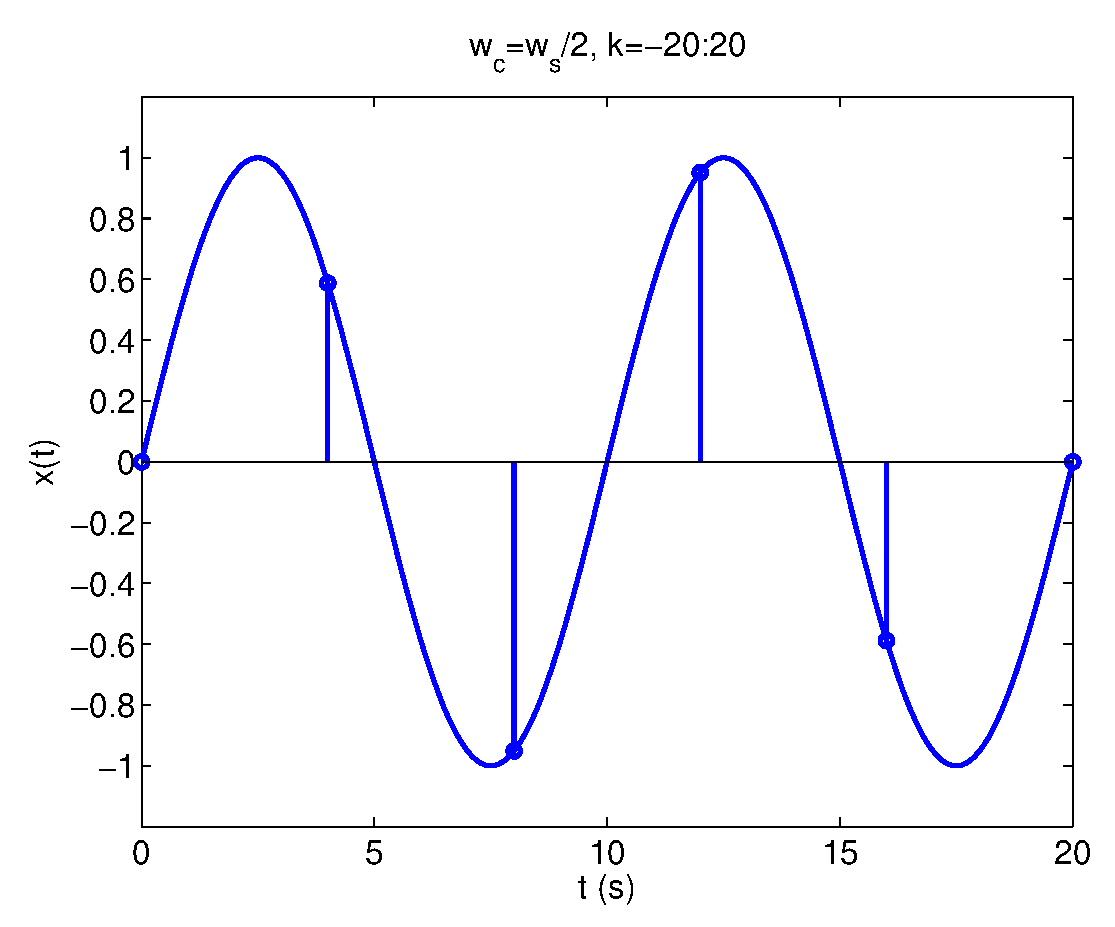
\includegraphics[width=4.3cm]{./Figures/RecIdealEjem1_1.eps}}\only<5|handout:0>{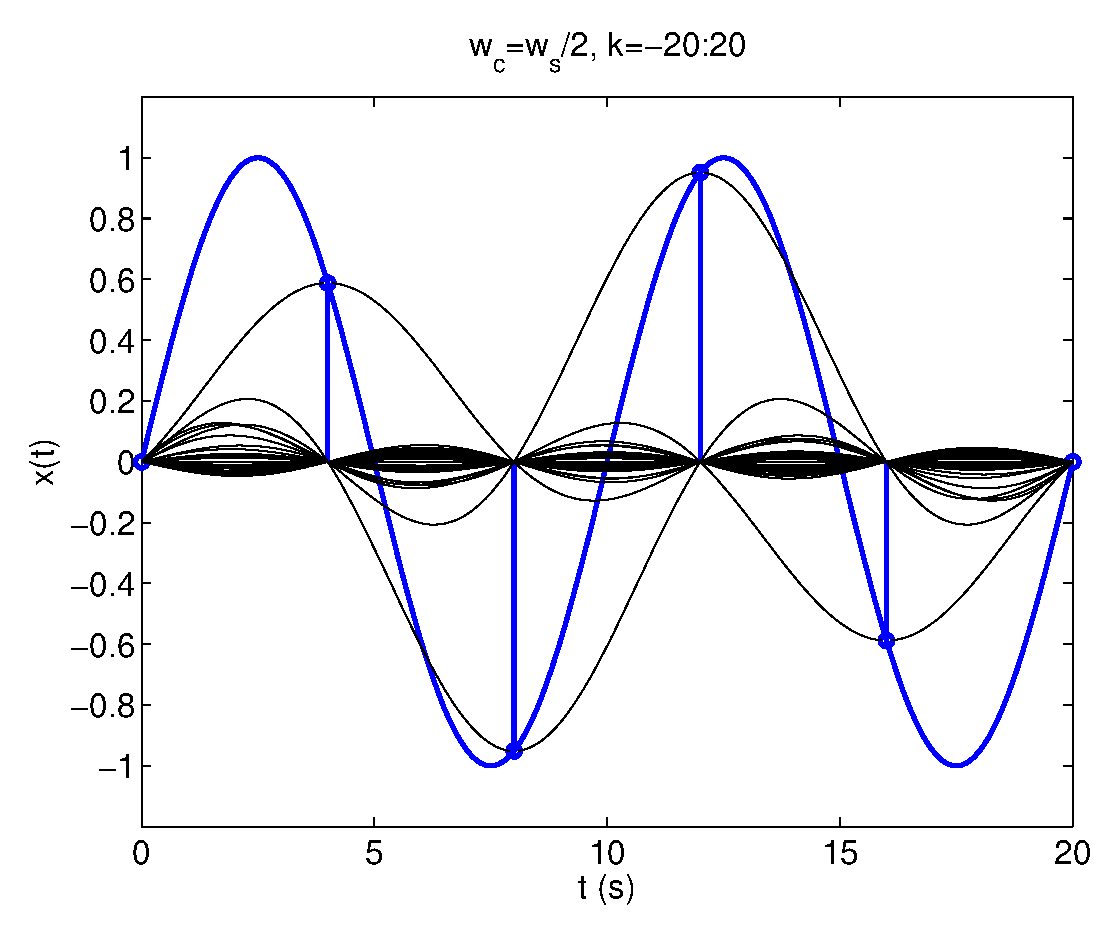
\includegraphics[width=4.3cm]{./Figures/RecIdealEjem1_2.eps}}\only<6->{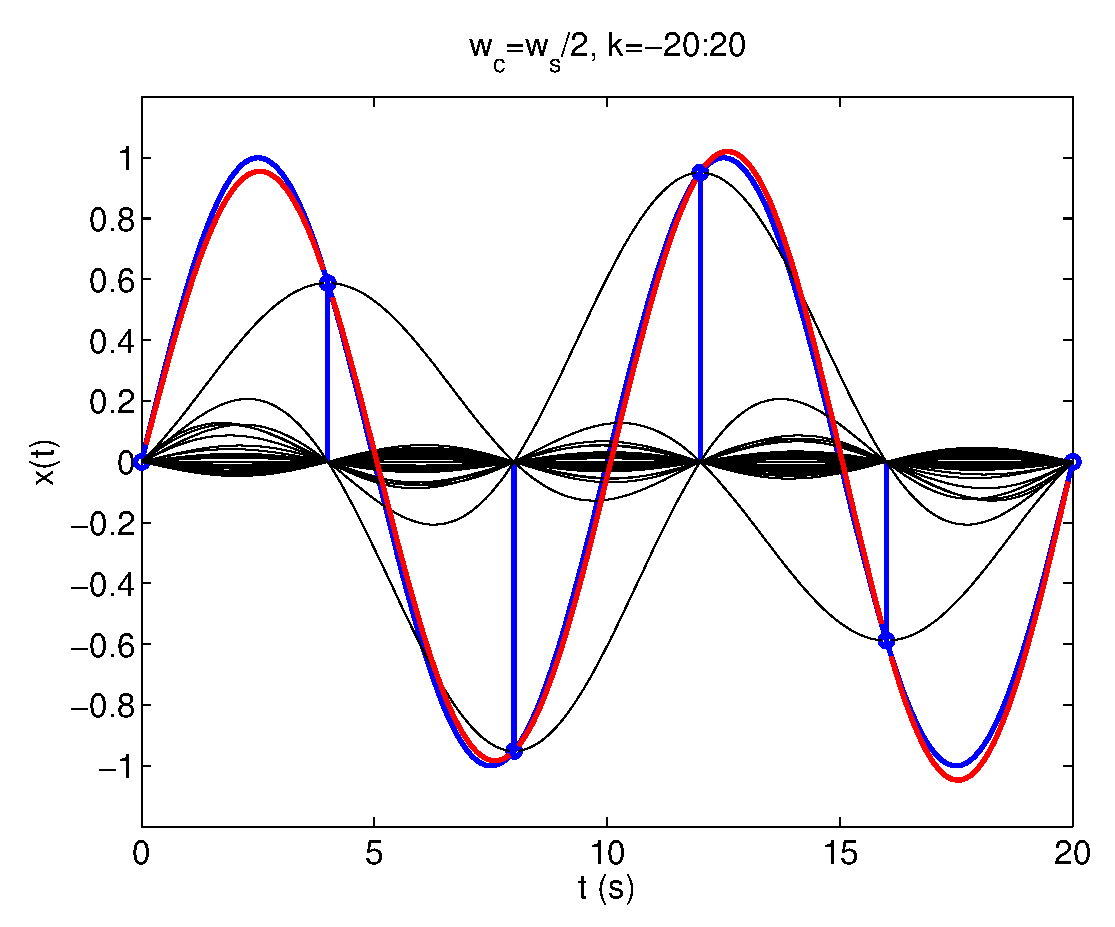
\includegraphics[width=4.3cm]{./Figures/RecIdealEjem1_3.eps}}
\end{column}
\begin{column}{5cm}
\only<7|handout:0>{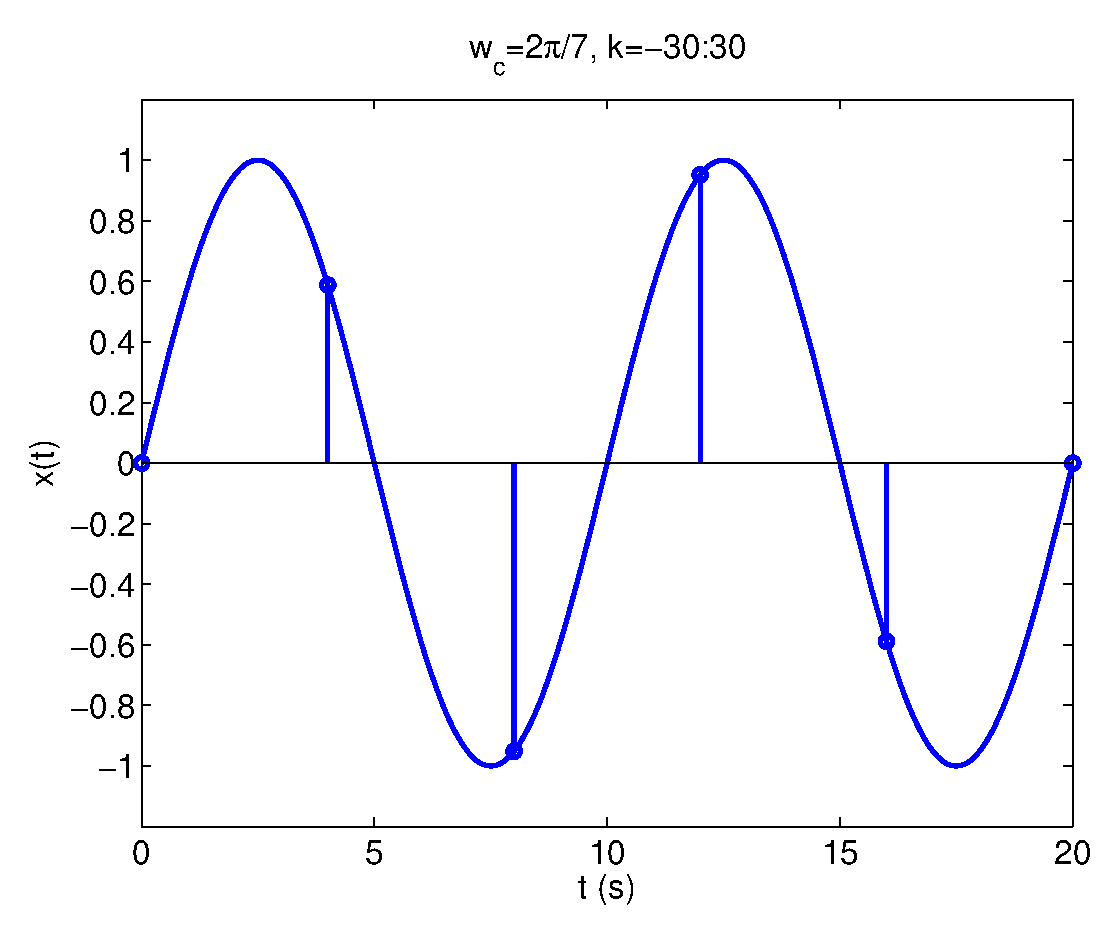
\includegraphics[width=4.3cm]{./Figures/RecIdealEjem2_1.eps}}\only<8|handout:0>{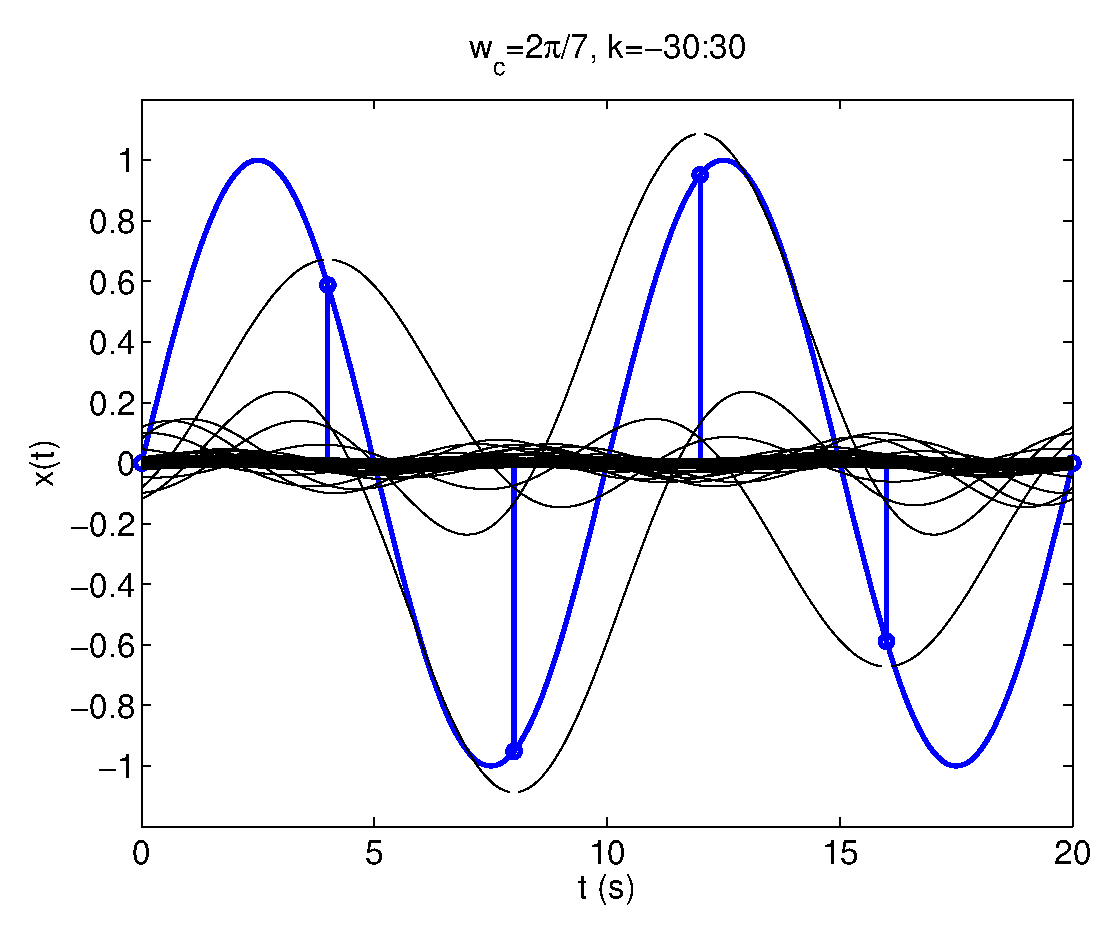
\includegraphics[width=4.3cm]{./Figures/RecIdealEjem2_2.eps}}\visible<9->{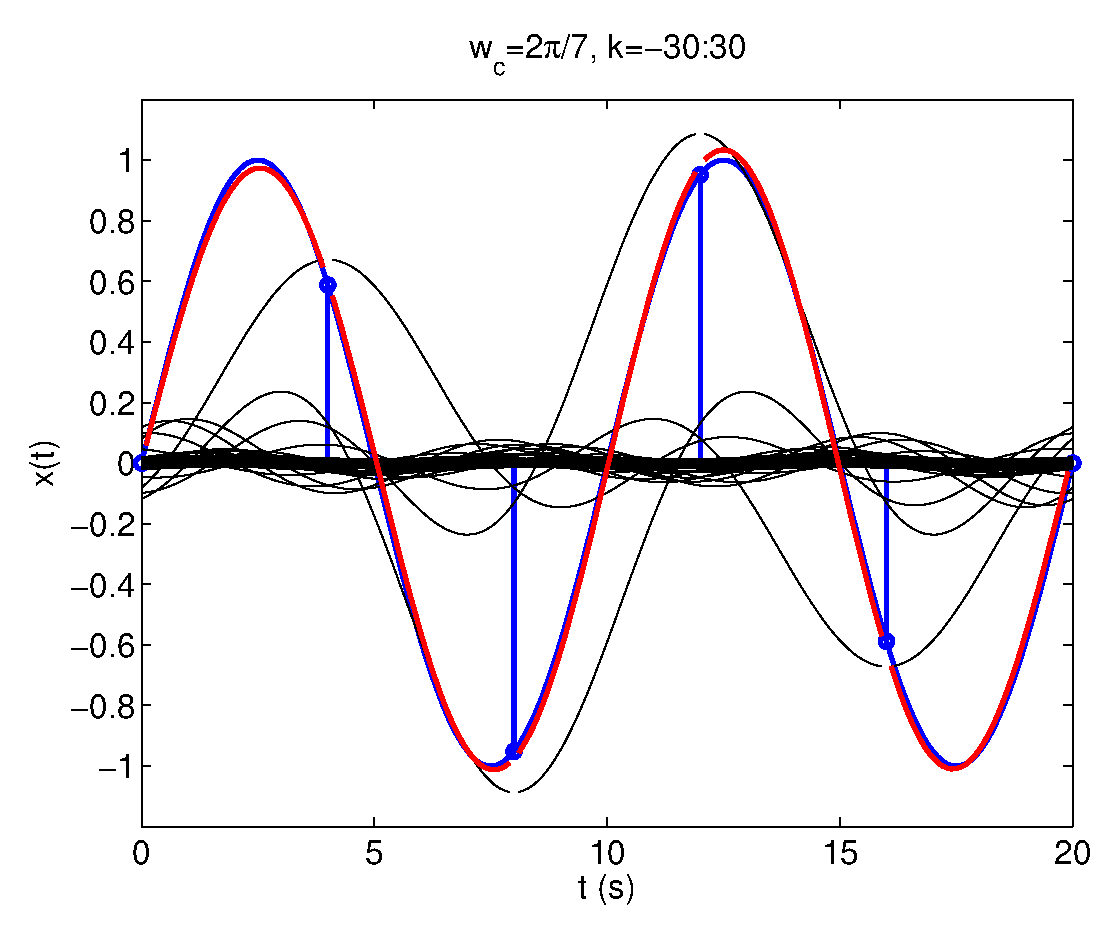
\includegraphics[width=4.3cm]{./Figures/RecIdealEjem2_3.eps}}
\end{column}
\end{columns}

\end{frame}

\subsection{Reconstrucción mediante interpolación}

\begin{frame}
\frametitle{Reconstrucción mediante interpolación I}

\footnotesize 
\begin{itemize}
\item Aunque la reconstrucción a través de un filtro paso baja ideal se puede considerar un método de interpolación de las infinitas muestras de la señal, ésta no se puede realizar de forma computacionalmente eficiente.
\item Por lo tanto, se utilizan métodos alternativos, más sencillos en los que únicamente se interpolan un número finito de muestras:
\begin{itemize}
\footnotesize 
\item Retenedor de orden cero (zero-order holder, ZOH): mantiene constante el valor de la muestra hasta el instante siguiente.
\item Retenedor de orden uno (first-order holder, FOH): interpola lineamente entre dos muestras sucesivas.
\item Retenedor de orden dos (second-order holder, SOH): interpola cuadraticamente entre tres muestras sucesivas.

\end{itemize}

\item Ninguno de estos interpoladores permiten reconstruir totalmente la señal, ya que modifican el espectro en frecuencia de la señal muestreada que los atraviesa. Para verlos los cambios en frecuencia de la señal, podemos analizar el espectro de los retenedores.

\end{itemize}
\end{frame}

\begin{frame}
\frametitle{Reconstrucción mediante interpolación II}

\footnotesize

\vspace{-0.1cm}

\hspace{1.0cm}{$x_p(t)\!= \! \sum_{k=-\infty}^{\infty}x_c(t)\delta(t-kT_s)$}  \hspace{0.3cm} y \hspace{0.3cm} {$X_p(jw)\!\!=\!\!\frac{1}{T_s}\!\! \sum_{k=-\infty}^{\infty}\!X_c(j(w\!-\!kw_s))$}

\rule{11cm}{0.4pt}

\begin{columns}[c]
\begin{column}{4.5cm}
\footnotesize

\vspace{-0.9cm}

\begin{itemize}
\item Retenedor de orden cero:
\end{itemize}

 \begin{figure}
  \centering
  \small
\scalebox{0.8}{
  \begin{psmatrix}[mnode=r,colsep=0.5,rowsep=0.3]
  [name=inc1] &&& &[name=continuo]  \visible<1-> {\psframebox[fillstyle=solid,fillcolor=yellow,framesep=2pt,linecolor=gray,linewidth=0.4pt]{\parbox[c]{8ex}{\centering ZOH}}} & &&&  [name=ind2]\\
     \visible<1->{\ncline[linecolor=black]{->}{inc1}{continuo}  \Bput{$\delta(t)$}\Aput{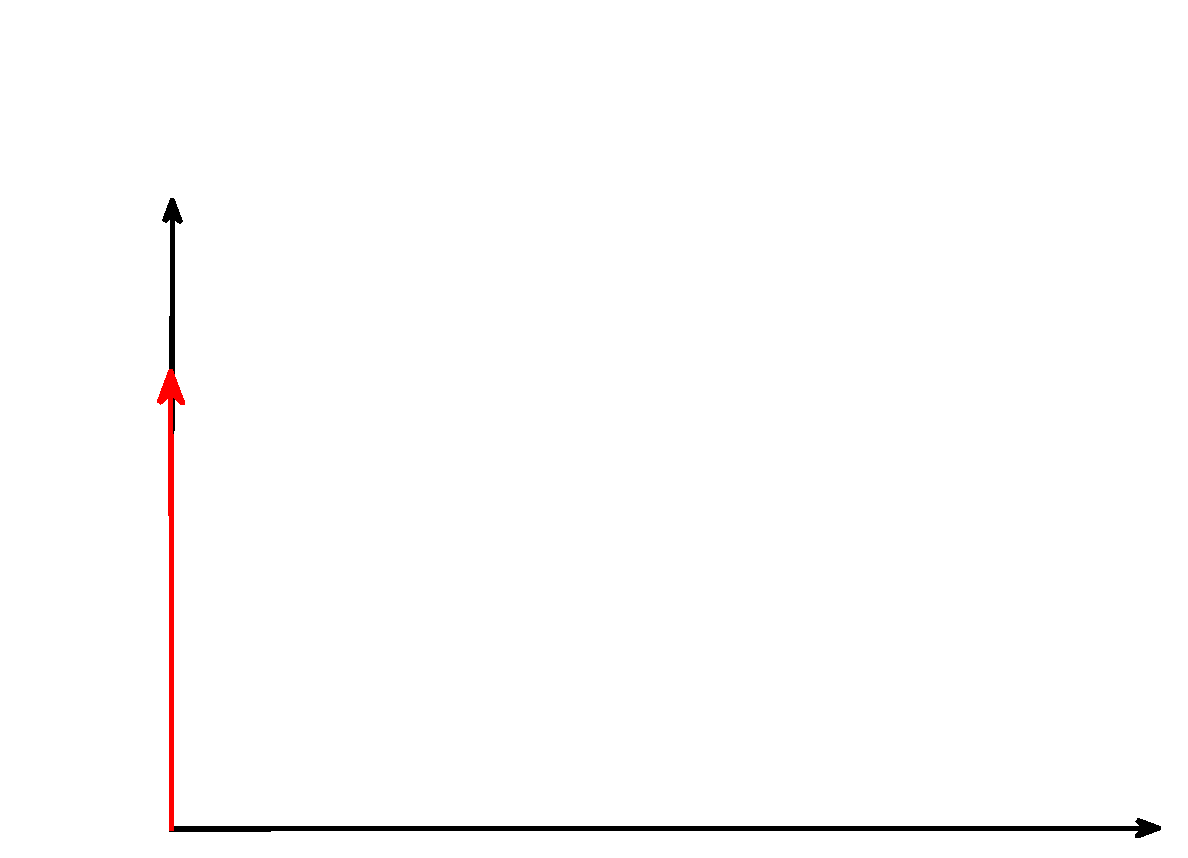
\includegraphics[width=1.5cm]{./Figures/inputimp.eps} }}
   \visible<1->{\ncline[linecolor=black]{->}{continuo}{ind2}  \Bput{h(t)}\Aput{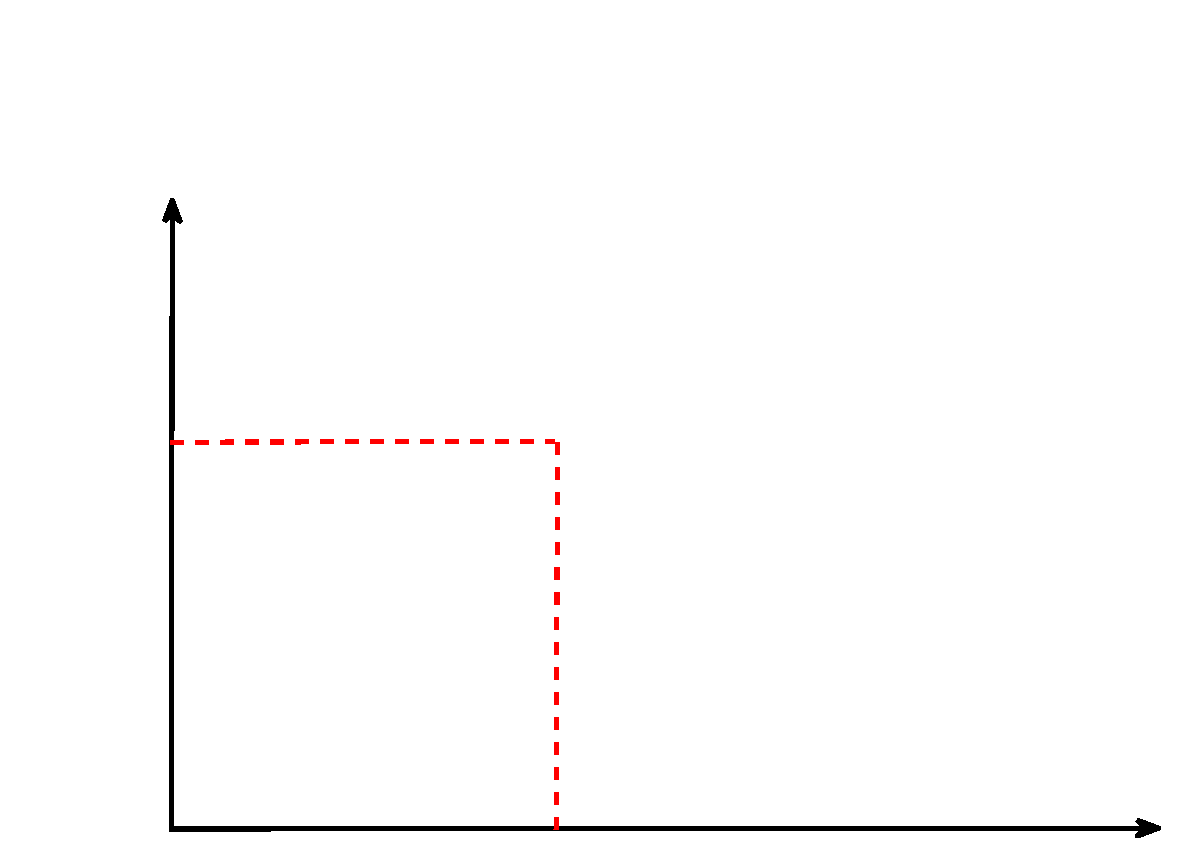
\includegraphics[width=1.5cm]{./Figures/outputimp.eps} }}
%\visible<1->{\ncline[linecolor=black]{-}{ind1}{jjj} }
    \end{psmatrix}  
  }
\end{figure}

\vspace{-0.4cm}
\visible<2->{
\begin{itemize}
\item Retenedor de orden uno:
\end{itemize}

 \begin{figure}
  \centering
  \small
\scalebox{0.8}{
  \begin{psmatrix}[mnode=r,colsep=0.5,rowsep=0.3]
  [name=inc1] &&& &[name=continuo]  \visible<1-> {\psframebox[fillstyle=solid,fillcolor=yellow,framesep=2pt,linecolor=gray,linewidth=0.4pt]{\parbox[c]{8ex}{\centering FOH}}} & &&&  [name=ind2]\\
     \visible<1->{\ncline[linecolor=black]{->}{inc1}{continuo}  \Bput{$\delta(t)$}\Aput{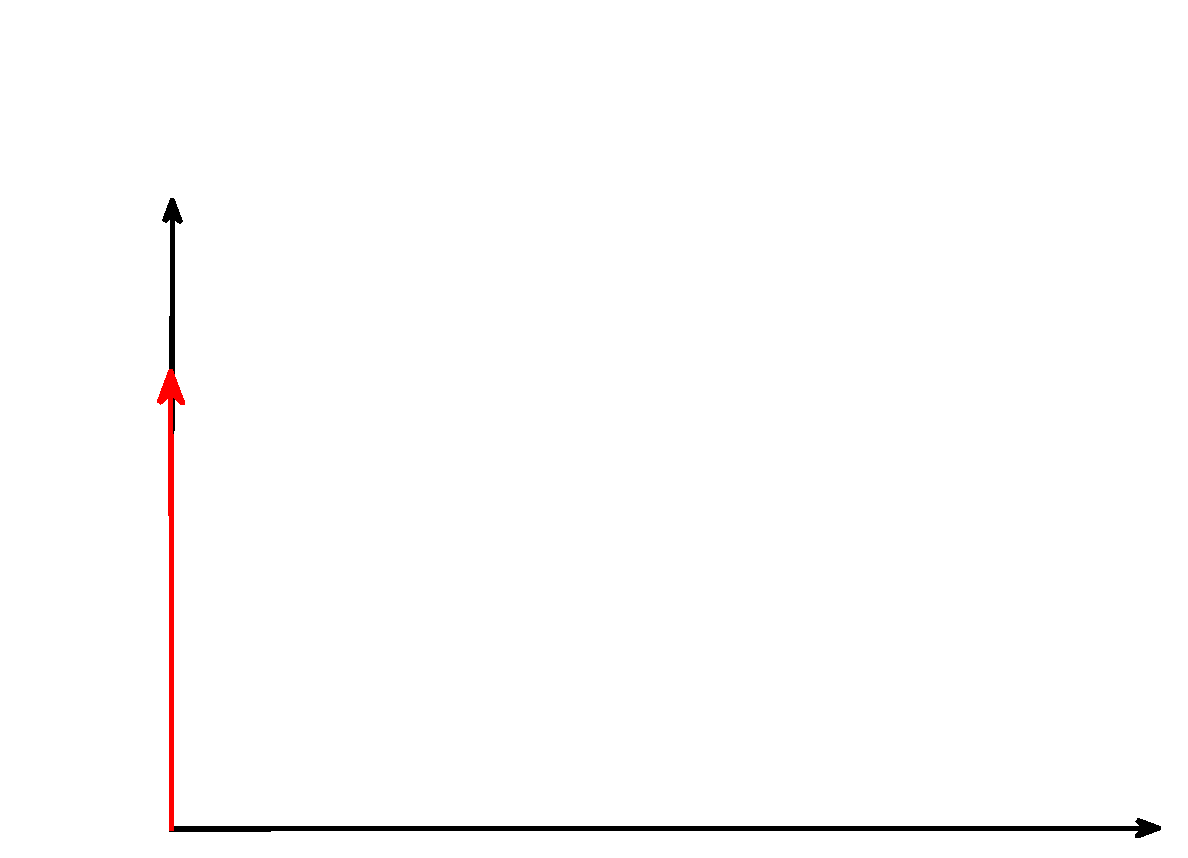
\includegraphics[width=1.5cm]{./Figures/inputimp.eps} }}
   \visible<1->{\ncline[linecolor=black]{->}{continuo}{ind2}  \Bput{h(t)}\Aput{}}
%\visible<1->{\ncline[linecolor=black]{-}{ind1}{jjj} }
    \end{psmatrix}  
  }
\end{figure}

\vspace{-0.5cm}
}
\visible<3->{
\begin{itemize}
\item Filtro paso bajo ideal:

(con $w_c=\frac{w_s}{2}$)
\end{itemize}
}

\end{column}
\begin{column}{6cm}

$h(t)=\Pi(\frac{t-T_s/2}{T_s})$  

\vspace{0.1cm}

$y(t)=(h*x_p)(t)=$

\vspace{0.1cm}

\hspace{0.7cm}$=\sum_{k=-\infty}^{\infty}x_c(kT) \Pi(\frac{t-T_s/2-kT_s}{T_s})$

\vspace{0.1cm}

$H(jw)=e^{jw\frac{T_s}{2}} T_s Sa(T_s w/2)$

\vspace{0.1cm}

\rule{5cm}{0.4pt}

\visible<2->{
$h(t)=\Lambda(\frac{t}{T_s})$  

\vspace{0.1cm}

$y(t)=(h*x_p)(t)=$

\vspace{0.1cm}

\hspace{0.7cm}$=\sum_{k=-\infty}^{\infty}x_c(kT) \Lambda(\frac{t-kT_s}{T_s})$

\vspace{0.1cm}

$H(jw)=T_s Sa^2(T_s w/2)$

\vspace{0.1cm}

%%%%%%%%%%%%%%%%%%%%
%%%%%%%%%%%%%%%%%%%%
\rule{5cm}{0.4pt}}

\visible<3->{
\vspace{0.1cm}

\footnotesize

$h(t)=Sa(\frac{w_s t}{2})$

\vspace{0.1cm}

$y(t)\!=\!\! \sum_{k=-\infty}^{\infty} \!x_c(kT_s) Sa(\frac{w_s(t\!-\!kT_s)}{2})$ 

\vspace{0.1cm}

$H(jw)=T_s \Pi(\frac{w}{w_s})$

\vspace{0.0cm}
}



\end{column}
\end{columns}



\end{frame}

\begin{frame}
\frametitle{Reconstrucción mediante interpolación III}


\begin{columns}[c]
\begin{column}{5cm}
\includegraphics[width=5cm]{./Figures/RecIdeal.ps}
\end{column}
\begin{column}{7cm}
\begin{itemize}
\footnotesize
\item Retenedor orden cero:
$H(jw)=e^{jw\frac{T_s}{2}} T_s Sa(T_s w/2)$

\item Retenedor orden uno:
$H(jw)=T_s Sa^2(T_s w/2)$

\item Filtro ideal:

$H(jw)=T_s \Pi(\frac{w}{w_s})$
\end{itemize}

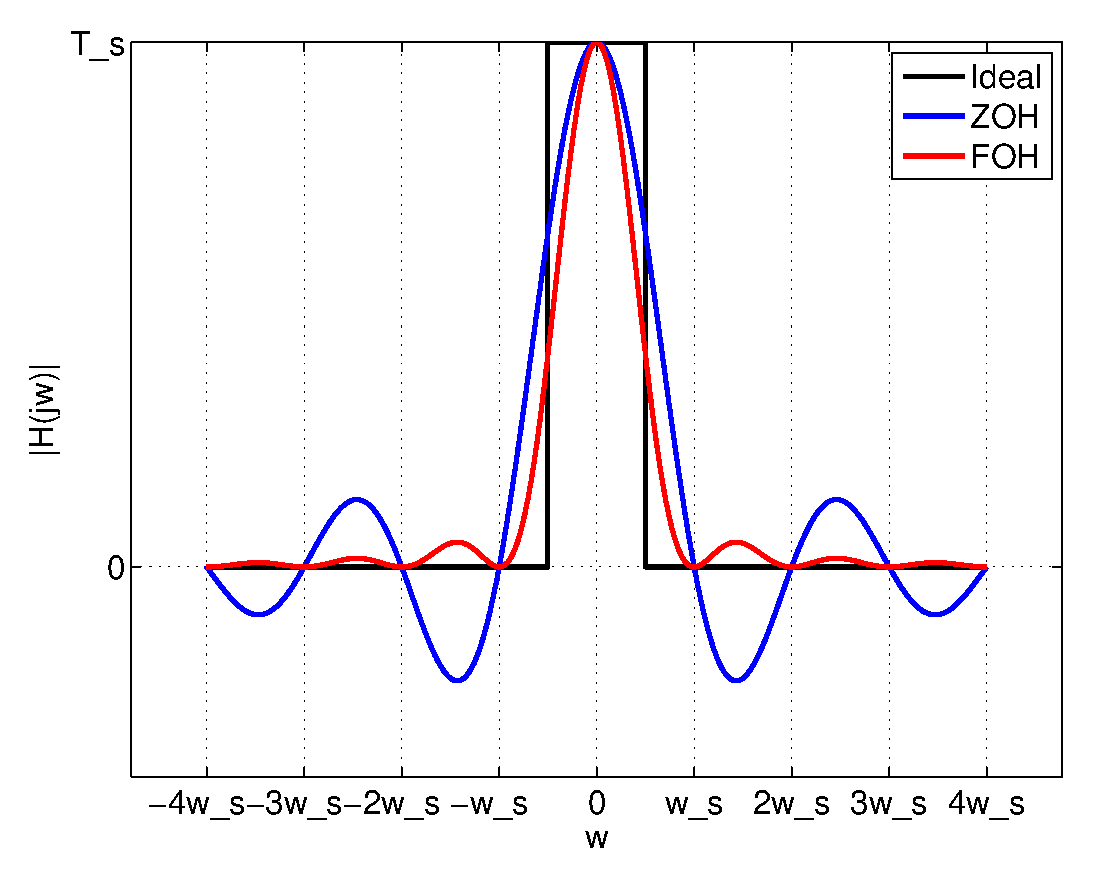
\includegraphics[width=4.5cm]{./Figures/Interpolacion.eps}

\end{column}
\end{columns}


\end{frame}


\begin{frame}
\frametitle{Retenedor de orden uno (FOH)}

\footnotesize

\begin{columns}[c]
\hspace{-0.6cm}\begin{column}{8cm}
\begin{itemize}
\item Versión no causal : 
\begin{itemize}

\footnotesize

\item $h(t)=\Lambda(\frac{t}{T_s})$

\item $y(t)=\sum_{k=-\infty}^\infty x_c(kT)\Lambda(\frac{t-kT_s}{T_s})$

\visible<3->{

\vspace{0.1cm}

\item Es no causal porque:

\begin{itemize}

\item Durante el periodo $t \in (kT_s,(k\!+\!1)T_s)$:  $y(t)=x_c(kT)+\frac{x_c((k+1)T)-x_c(kT)}{T_s} (t-kT_s)$. Depende de un valor fúturo. 

\item Su h(t) toma valores no nulos en instantes previos a t=0.

\end{itemize}
}

\end{itemize}

\visible<4->{

\item Versión causal: }

\begin{itemize}
\footnotesize
\visible<4->{\item Durante el periodo $t \in (kT_s,(k\!+\!1)T_s)$: $y(t)=x_c(kT)+\frac{x_c(kT)-x_c((k-1)T)}{T_s} (t-kT_s)$}

\vspace{0.1cm}

\visible<6->{
\item $h(t)=\Pi(\frac{t-T_s/2}{T_s})(1+\frac{t}{T_s})-\Pi(\frac{t-3T_s/2}{T_s})\frac{t-T_s}{T_s}$}

\vspace{0.1cm}
\visible<7->{
\item Se puede calcular el espectro del filtro (Matlab)}
\end{itemize}


\end{itemize}
\end{column}
\hspace{-0.6cm}\begin{column}{4cm}
\only<1|handout:0>{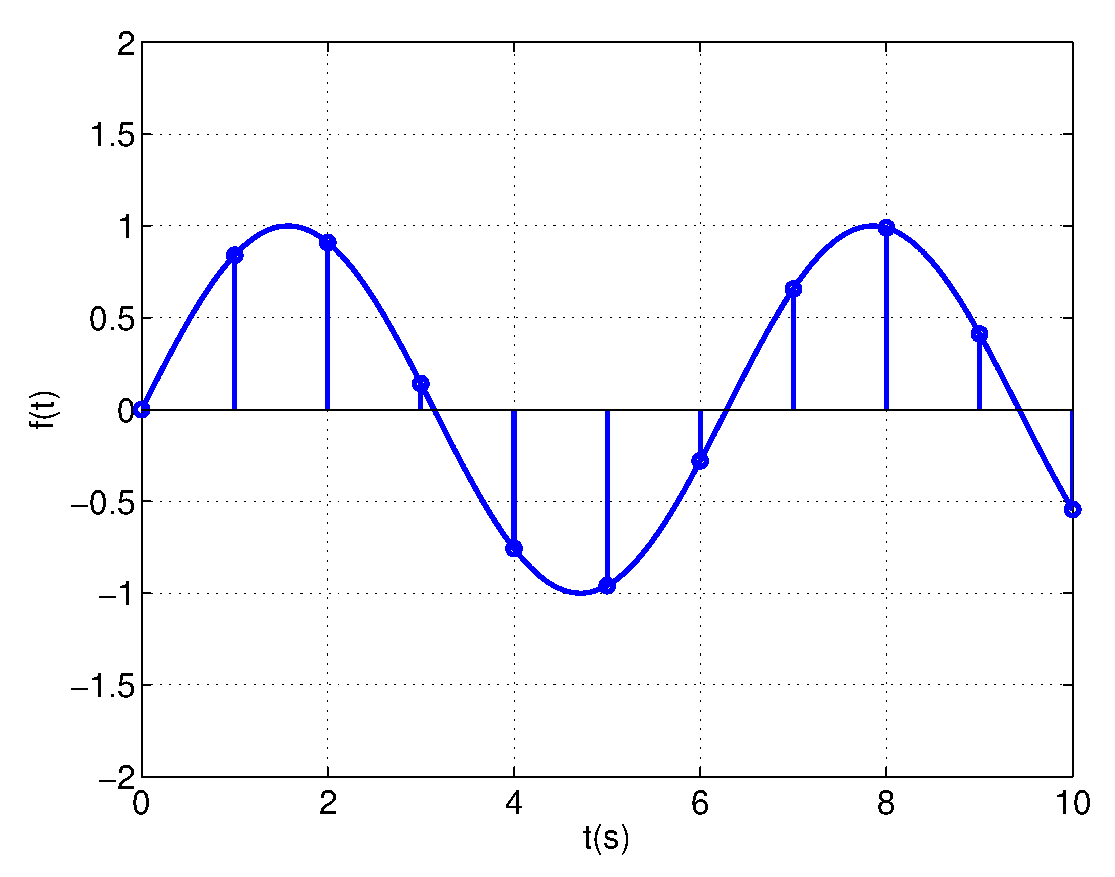
\includegraphics[width=4.5cm]{./Figures/FOHsTime0.eps}}\only<2-4|handout:0>{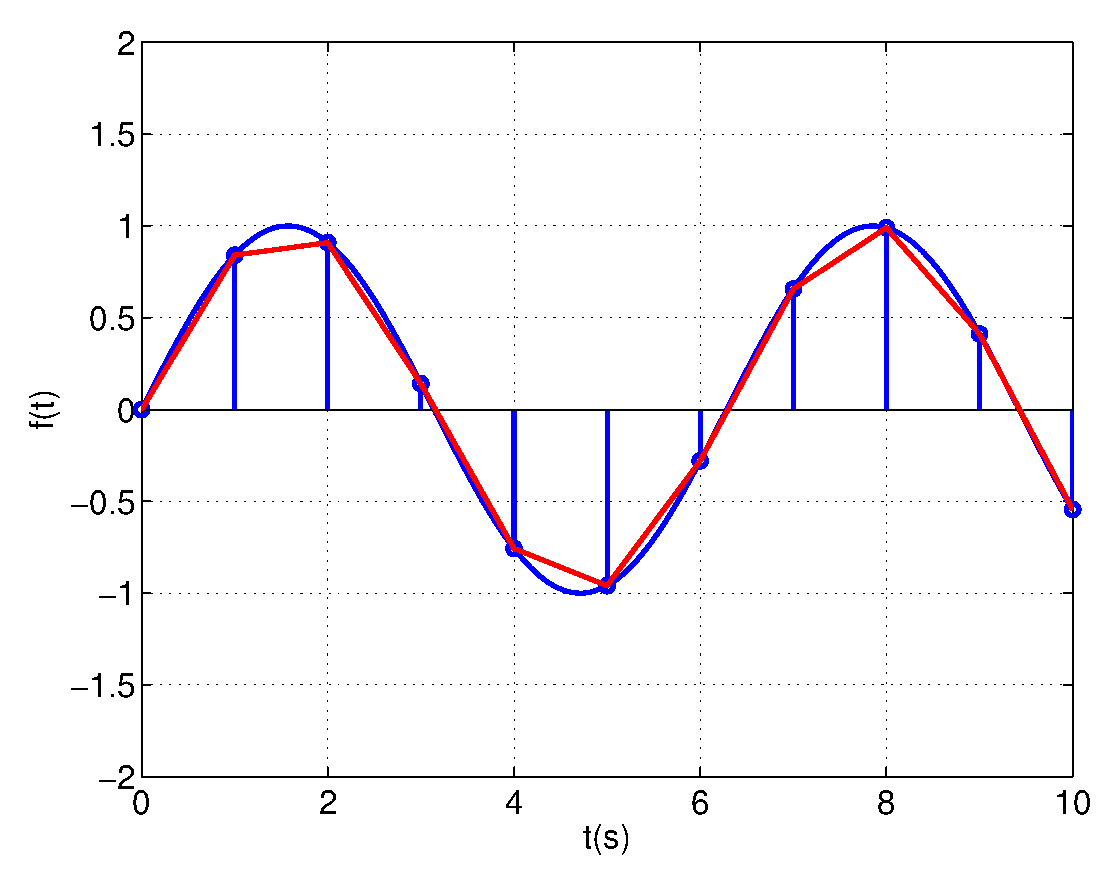
\includegraphics[width=4.5cm]{./Figures/FOHsTime1.eps}}\only<5->{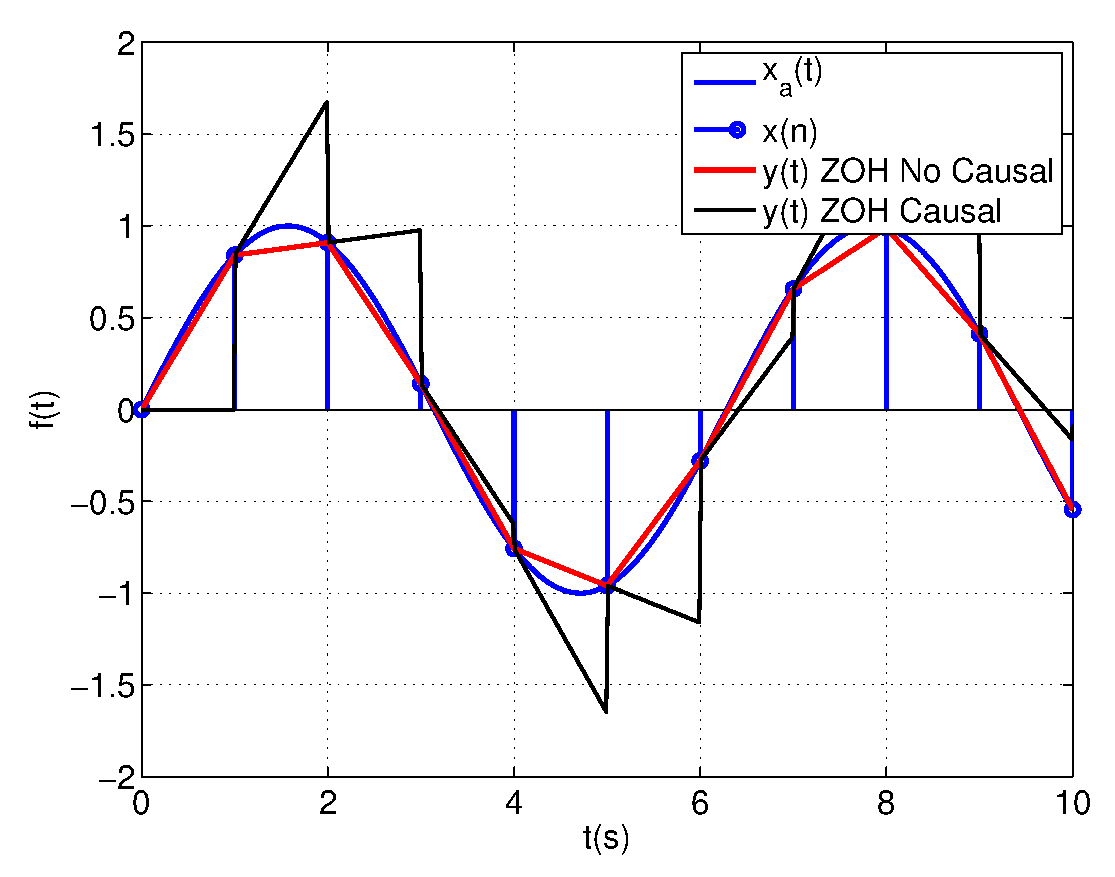
\includegraphics[width=4.5cm]{./Figures/FOHsTime.eps}}

\visible<8->{
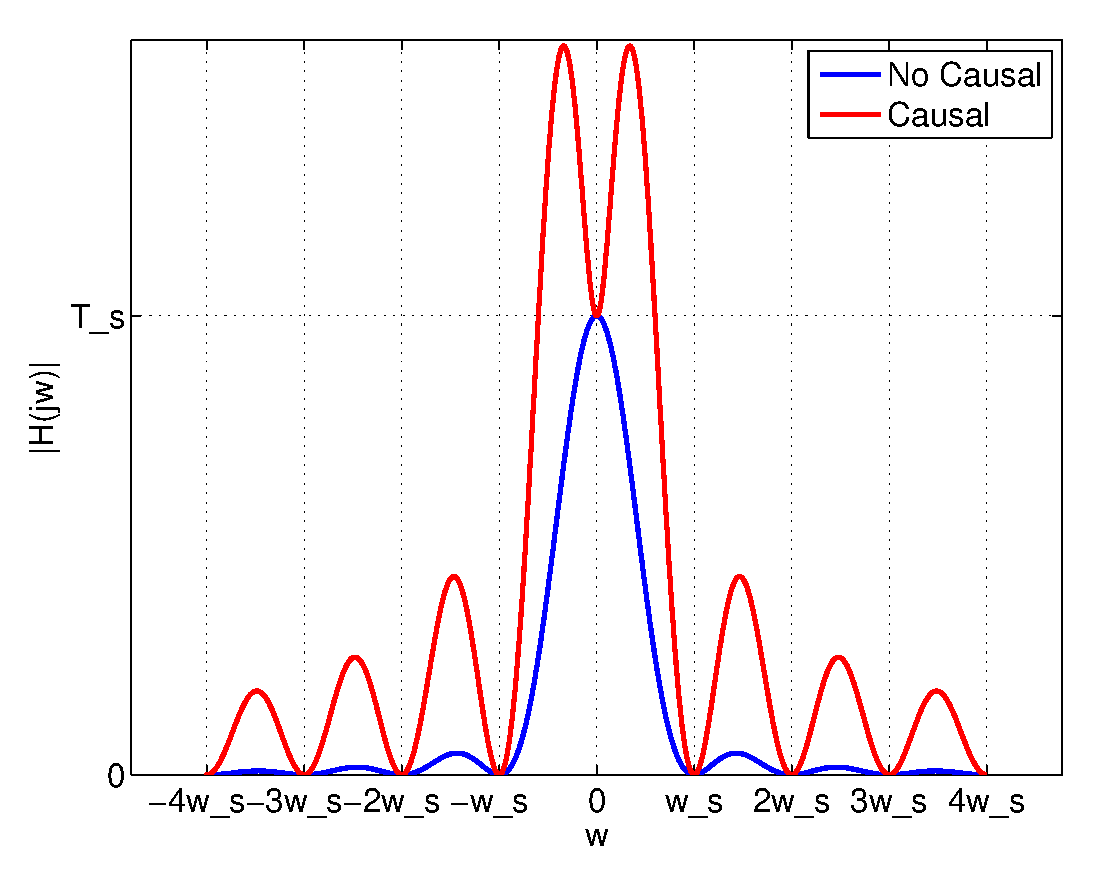
\includegraphics[width=4.5cm]{./Figures/FOHsFrec.eps}}

\end{column}
\end{columns}
\end{frame}
